\documentclass[../main.tex]{subfiles}
\begin{document}
\section{Meta-heuristic Optimization}
\label{sec:meta_heuristic}	

\subsection{Idea and motivation}

	As mentioned above, there are four kinds of nature-inspired meta-heuristic algorithms. They are evolution-based, physics-based, swarm-based and human-based optimization algorithms.
	
	Evolution-based methods are those that optimize following evolutionary rules in nature. The process starts with a ramdomly generated individual considered as population, being enhanced through each generation. Each generation commonly contains the following components: reproduction, fitness evaluation and selection. Specifically, in the reproduction process, from which new-born solutions are generated, often adopts generic operators such as crossover or mutation; the fitness evaluation process obtains the quality of each solution in current population by assigning their fitness values; and selection process is willing to determine candidates with superior values among the population to survive in the next generation. The strength point of this kind of algorithms is that the best individuals are always chosen to generate potential candidate for the subsequent generation. This move the population towards and come closer to the optimal value. The most popular evolution-based algorithm is Generic Algorithm (GA) \cite{holland1992genetic}, which mathematically mimicks the Darwinian's evolutionary laws. Other later algorithms are Generic Programming (GP) \cite{koza1997genetic}, Differential Evolution (DE) \cite{fleetwood2004introduction}, Biogeography-based optimization (BBO) \cite{simon2008biogeography} and Coral Reefs Optimization Algorithm (CRO) \cite{salcedo2013novel}. 
	
\begin{table}[!t]
\caption{Swarm-based optimization algorithms developed in literature.}
\label{tbl_swarm_algos}
\centering
\begin{tabular}{|p{6cm}|p{4cm}|p{2cm}|}
 \hline
 Algorithms & Inspiration & Year of proposal  \\ 
 \hline
Particle Swarm Optimization (PSO) \cite{eberhart1995particle} & bird blocks and fish schools & 1995 \\ \hline
Ant Colony Optimization (ACO) \cite{dorigo1999ant} & Ant colony & 1999 \\ \hline
Honey Bees Optimization Algorithm (HBO) \cite{abbass2001mbo} & Marriage in honey bee & 2001 \\ \hline
Bacterial Foraging Optimization (BOA) \cite{passino2002biomimicry} & Bacterial foraging behaviors & 2002 \\ \hline
Artificial Bee Colony (ABC\cite{basturk2006artificial} & Bee colony & 2005 \\ \hline
Firefly algorithm (FA) \cite{yang2009firefly} & Firefly swarm & 2009 \\ \hline
Bat Algorithm (BA) \cite{yang2012bat} & Bat swarm & 2012 \\ \hline
Dolphin Echolocation Algorithm (DEA) \cite{kaveh2013new} & echolocation behavior of Dolphins & 2013 \\ \hline
Grey Wolf Optimizer (GWO) \cite{mirjalili2014grey} & Wolf clan hierachy & 2014 \\ \hline
Whale Optimization Algorithm (WOA) \cite{mirjalili2016whale} & Humppack whale hunting behaviors & 2016 \\ \hline
Lion Optimization Algorithm (LOA) \cite{yazdani2016lion} & Lion hunting activities & 2016 \\ \hline
Seagull optimization algorithm (SOA) \cite{dhiman2019seagull} & Seagull swarm & 2019 \\ \hline
Sea Lion Optimization (SLnO) \cite{masadeh2019sea} & Sea lion hunting & 2019 \\ \hline


 \hline
\end{tabular}
\end{table}
	
	Physics-based methods try to mimic physical phenomena, and find a way to reach the optimal values following these principles. There are several popular algorithms in this category including Big-Bang Big-Crunch(BBBC) \cite{erol2006new}, Gravitational Search Algorithm (GSA) \cite{rashedi2009gsa}, Charged System Search (CSS) \cite{kaveh2010novel}, Central Force Optimization (CFO) \cite{formato2007central}, Artificial Chemical Reaction Optimization Algorithm (ACROA) \cite{alatas2011acroa}, Black Hole (BH) algorithm \cite{hatamlou2013black}, Ray Optimization (RO) algorithm \cite{kaveh2012new}, Small-World Optimization Algorithm
(SWOA)  \cite{du2006small}.
	
	Swarm Intelligence (SI) or swarm-based optimization is a group of algorithms being inspired by living and foraging behaviors of animals in the nature. Unlike evolution-based methods, SI methods are based on artificial search agents' movement in a pre-defined search space. Such algorithms take advantages of exploration and exploitation phases and lead the population closer and closer to the optimal result over the course of iteration. For example, one of the most famous and widely used algorithm in SI group is Particle Swarm Optimization (PSO) \cite{eberhart1995particle}, which uses the information both from the best agent and all the agents' best experience to search for the optima of a fitness function. Another popular swarm-based algorithm is Ant Conoly Optimization (ACO) \cite{dorigo1999ant}, which is inspired by social foraging process of ants. This algorithm uses the idea of the social intelligence of ants in finding the closest path from the nest and a source of food. A pheromone matrix is
enhanced over the course of iteration by the candidate solutions.  Several other SI algorithms have been regularly proposed, some of them are listed in Table. \ref{tbl_swarm_algos}. In general, this group of methods started to become more attractive since PSO is proven to be very competitive with evolution-based and physics-based algorithms. In fact, swarm-based methods have some advantages over the others. For example, swarm-based algorithms find new better by preserving the information from previous iterations, while evolution-based methods such as GA discard any information immediately when a new generation is formed. Also, they are usually formed of less updating operators compared to the others (crossover, mutation, selection $etc.$) and therefore it is easier to implement.


	Human-based algorithms are recently developed by observing and applying human behaviors in daily life. Some of the well-known algorithms are Harmony Search (HS) \cite{geem2001new}, Teaching Learning Based Optimization (TLBO) \cite{rao2011teaching}, League Championship Algorithm (LCA) \cite{kashan2014league}, Tabu Search (TS) \cite{de1989tabu} and Colliding Bodies Optimization (CBO) \cite{kaveh2014colliding}. 
\subsection{Particle Swarm Optimization (PSO)}
\label{pso_standard}
PSO~\cite{kennedy2010particle} is a very first swarm-based optimization, which is the premise of many other algorithms proposed in recent years. It emulates the behaviors of birds, fish and so forth when they forage for food and communicate as a swarm. In PSO system, a swarm contains several candidate solutions (also known as particles), which coexist in the search space of the problem with $D$ dimensions. The solution often cooperate and fly together to land on personal optimal positions. Over the course of time, the best personal position (its own best position in the past) of each particle and the global best position (the current best position of entire swarm) are recorded. The next position of a particle is updated based on the personal best (cognitive behavior) and the global best (social communication). With this approach, PSO combines local search (through personal best) with global search (through global best) to balance exploitation and exploration processes. PSO operation workflow is presented in Figure~\ref{fig_pso_algo}.
	 
\begin{figure}[!ht] 
   \centering
   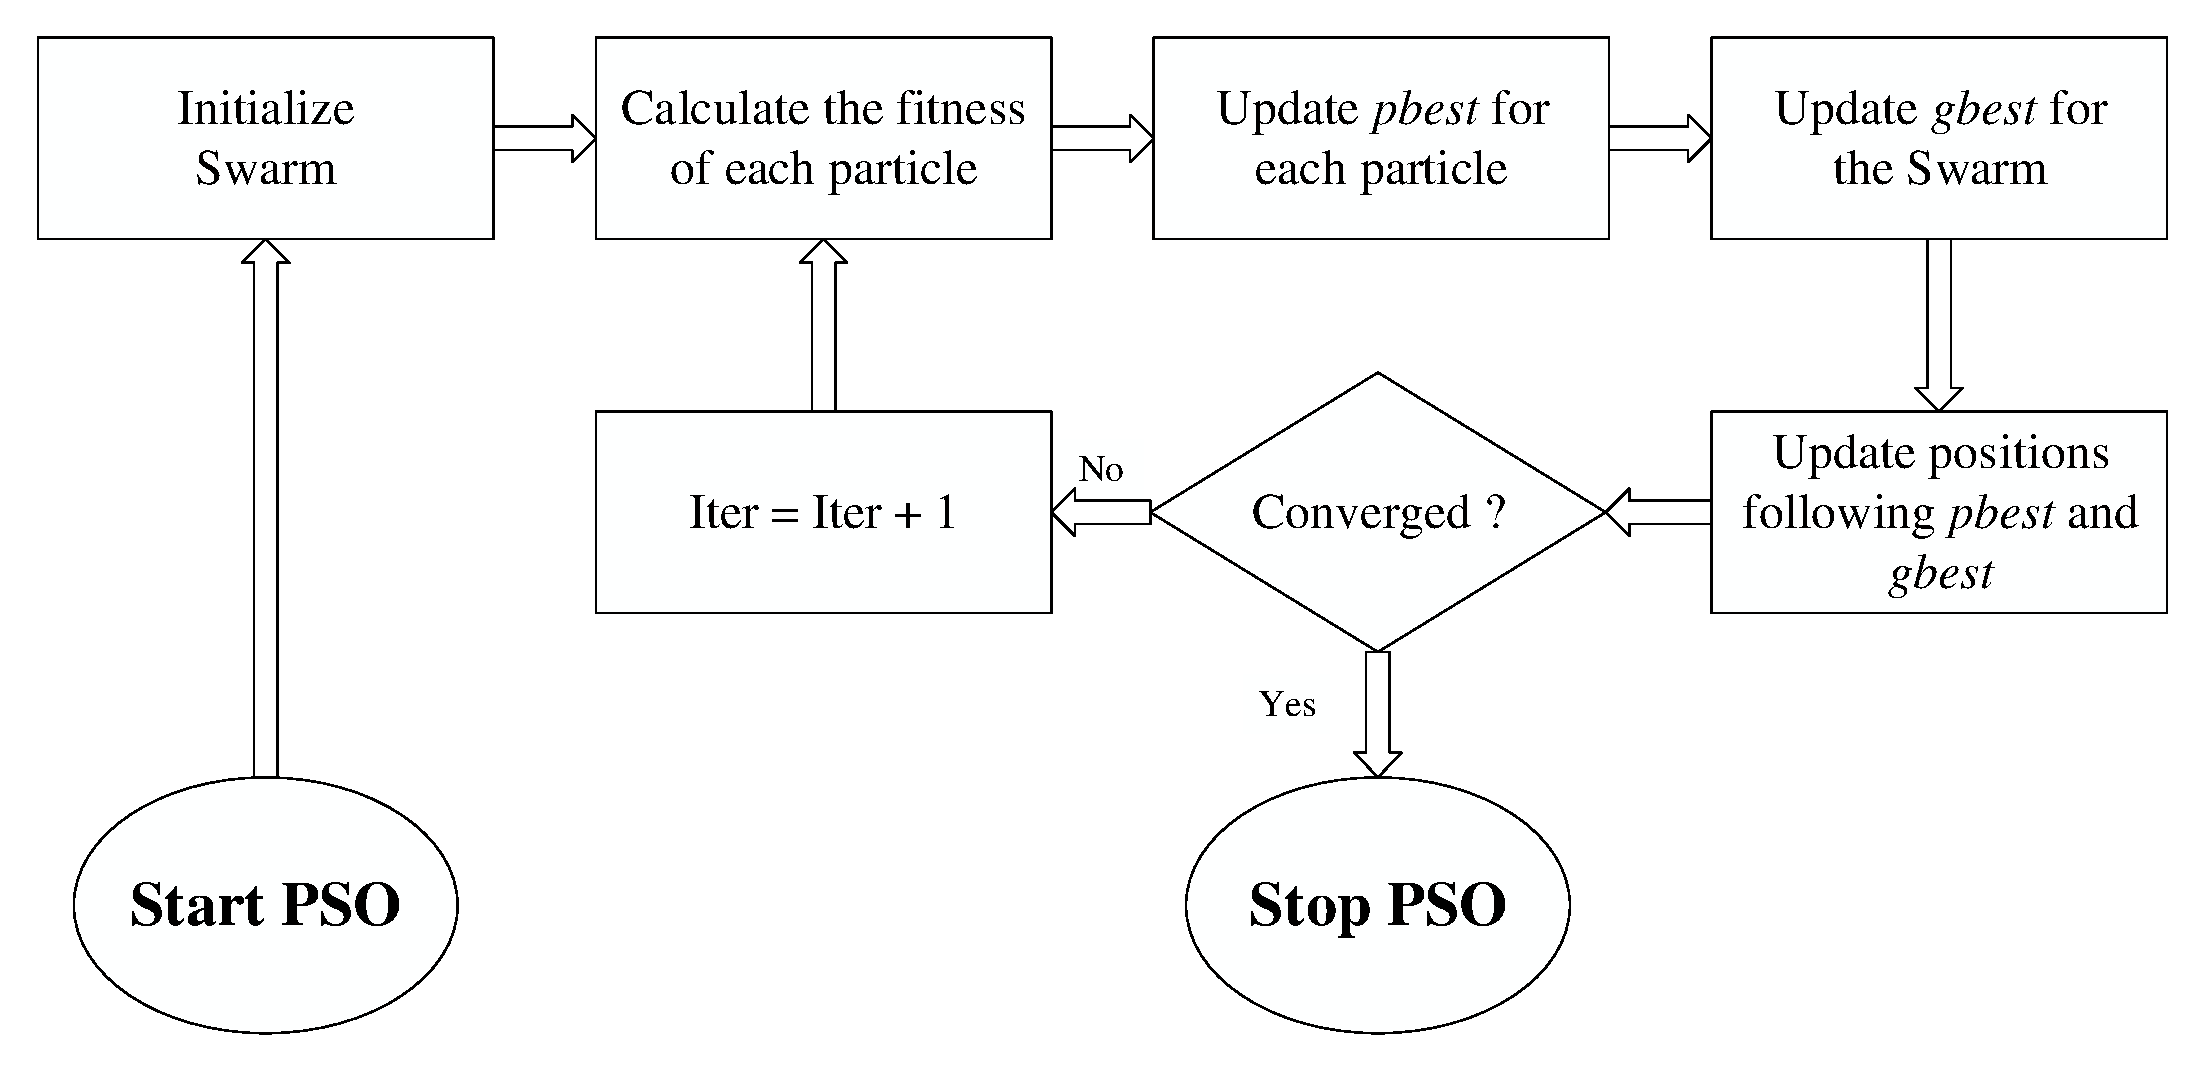
\includegraphics[width=0.75\linewidth]{pdf/model/pso}
  \caption{PSO flowchart} 
  \label{fig_pso_algo} 
\end{figure}
	 
Thus, each particle $i$ in swarm is described by two properties: its velocity $v_i$ and position $x_i$ in the search space. In each iteration, they are updated following the equation: 

\begin{equation} \label{eq_pso_1}
v_i^{t+1} = \omega.v_i^t + c_1.r_1(p_i^t - x_i^t) + c_2.r_2(g^t - x_i^t)
\end{equation}
\begin{equation} \label{eq_pso_2}
x_i^{t+1} = x_i^t + v_i^t
\end{equation}
where 
\begin{tabbing}
	xxx\=xxxxxxi\=\kill
	\>	$\omega$			\>	is inertia weight reduced linearly to zero through time; \\
	\>	$v_i^t$			\>	$v_i^t = [v_{i1}, v_{i2}, ..., v_{iD}]$ and is the velocity;	\\
	\>	$x_i^t$			\>	$x_i^t = [x_{i1}, x_{i2}, ..., x_{iD}]$ and is the position of 	\\
	\> 	\phantom{inv}	\> 	particle $i$ in current time $t$ respectively;\\
	\>	$p_i^t$			\>	is its personal best position in current time $t$; \\
	\>	$g^t$			\>	is global best position ever of entire swarm up to time $t$; \\
	\>	$c_1, c_2$ 		\>	are acceleration coefficients that pull particles \\
	\>	\phantom{inv} 	\>	faster to personal best and global best respectively;\\
	\>	$r_1, r_2$ 		\>	are random number which is uniformly distributed in $[0,1]$; \\
\end{tabbing}
\subsection{Sea Lion Optimization Algorithm (SLnO)}
\label{slno_standard} 
	
	The intelligence of sea lions can be seen through the way they organize their groups and hunt the prey. Hunting as a group allow sea lions to have more opportunities of obtaining more food especially when the amount of fish is quite large. Usually, sea lions capture their prey together by circling the prey in a narrow ball, and the size of this "ball" continues to be decrease until the prey is totally wiped out. The main phases of hunting behaviors of sea lions can be illustrated as 3 steps as follows:
	
\begin{algorithm}[!t]
\caption{Sea Lion Optimization (SLnO)}
\label{algorithm_slno}
\SetAlgoLined
 Initialize the Sea Lion population $X_i (i=1,2,.., n)$ randomly. \\
 Calculate fitness of each solution (sea lion). \\
 $X_*\gets$ the best solution \\
\For {$Iter=0 \to Iter_{max}$}{
	Calculate the value of $C$ \\
	\For {SeaLion in population}{\
		Calculate $SP_{leader}$ using Eq. \ref{snlo_eq3}  \\
		\uIf{$SP_{leader} < 0.25$}{
			\uIf {$|C| < 1$}{\
				Update the location of the current search agent using Eq. \ref{slno_eq1}
				}
			\Else {
				Choose a random search agent $SL_{rand}$ \\
				Update the locatiion of current search agent by Eq. \ref{slno_eq8} \\
			}
		}	
		\Else{
			Update the location of the current search agent by Eq. \ref{slno_eq6}
		}
	Evaluate population: fix if any solutions go beyond the boundary \\
 	Recompute the fitness of all solutions \\
 	Check and update $X_*$ if a better solution is found. \\
	}
	
}
 \textbf{Results:}  $X_*, f(X_*)$
\end{algorithm}
	
\begin{itemize}
\item Tracking and chasing the prey using their senses.
\item Calling other members to gather and implement encircling strategy around the prey.
\item Attack towards the prey which is captured in the circle.
\end{itemize}

	Those behaviors is the inspiration for the Sea Lion Optimization (SLnO) which was first introduced in ~\cite{masadeh2019sea}. The algorithm mimics the amazing social behaviors and interesting hunting activities of sea lions. The formulas of the phases \textit{Detecting and tracking phase}, \textit{Vocalization phase} and \textit{Attacking phase} illustrate perfectly encircling mechanisms which is utilized by sea lions. We summarize and discuss briefly each phase in the algorithm as below, meanwhile the pseudo-code of SLnO is provided in details in \textbf{Algorithm \ref{algorithm_slno}}.

\begin{enumerate}
\item \textbf{Detecting and tracking phase}

	Sea lions can identify the location of the prey and gather other members that will join the subgroup to organize the net following the encircling mechanism. In SLnO algorithm, the prey is considered as the current best solution or the solution closest to the optimal solution. This behaviors is presented mathematically using Eq. (\ref{slno_eq1}) and Eq. (\ref{slno_eq2}) as follows:
\begin{equation}\label{slno_eq1}
Dist = |2B.P(t) - SL(t)|
\end{equation}
\begin{equation}\label{slno_eq2}
SL(t+1) = P(t) - Dist.C
\end{equation}
	
	Where $Dist$ indicates the distance between the prey and the current sea lion; $P(t)$ and $SL(t)$ represent the position vectors of best solution and the sea lion in iteration $t$ respectively; $B$ is random vector in the range $[0, 1]$ which is multiplied by 2 to increase the search space. $SL(t+1)$ is the new position of search agent after updating and $C$ is linearly decreased from 2 to 0 over the course of iteration, indicating the encircling mechanism of sea lion group when they move towards the prey and surround them.

\item \textbf{Vocalization phase}
	
	When a sea lion recognize a group of their prey (such as fish), it will call other sea lions in their group for gathering and creating a net to capture the prey. That sea lion is considered as the leader and it will lead the group of sea lions moving towards and decide the behaviors of the group. These behaviors are modeled mathematically as shown in Eq. (\ref{snlo_eq3}), (\ref{snlo_eq4}) and (\ref{snlo_eq5}):
\begin{equation}\label{snlo_eq3}
SP_{leader} = |(V_1(1+V_2)/V_2|
\end{equation}
\begin{equation}\label{snlo_eq4}
V_1 = \sin(\theta)
\end{equation}
\begin{equation}\label{snlo_eq5}
V_2 = \sin(\phi)
\end{equation}
 Where $SP_{leader}$ is the value that illustrates the decision of the leader followed by other sea lions in the group; $\theta$ and $\phi$ are the angles of its voice's reflection and refraction in the water, respectively.
 
\item \textbf{Attacking phase (Exploitation phase)}
 
 The hunting activities of sea lions are led by the leader. In SLnO algorithm, the target prey is considered the current best candidate solution. In order to mathematically mimic the hunting behaviors of sea lions, two phases are introduced as follows:
 	
\begin{itemize}
\item \textit{Dwindling encircling technique:}
	This behavior depends on the value of $C$ in Eq. \ref{slno_eq2}. $C$ is linearly decreased from 2 to 0 over the course of iteration, so this allows the search space around the current best position to shrink and force other search agents to updated in this search space as well. Therefore, a new updated position of a sea lion can be located anywhere in the search space between its current position and the location of the present best agent.

\item \textit{Circling updating position}: Sea lions chase bait ball of fishes and hunt them starting from edges. Eq. \ref{slno_eq6} is proposed in this regard:
\begin{equation} \label{slno_eq6}
SL(t+1) = |P(t) - SL(t)|.\cos(2 \pi m) + P(t)
\end{equation}	
\end{itemize}
	Where $|P(t) - SL(t)|$ illustrates the distance between the best optimal solution (the prey) and the current search agent in t-th iteration, $||$ means the absolute value and $m$ is a random number in the range $[-1, 1]$.
	
\item \textbf{Searching for prey (Exploration phase)}
	In exploration phase, the search agents update their positions based on a randomly selected sea lion. The condition that allows exploitation phase to happen is when the value of $C$ becomes greater than 1, and the process of finding a new agent is presented by Eq. (\ref{slno_eq7}) and (\ref{slno_eq8}) as below:
\begin{equation}\label{slno_eq7}
Dist = |2B.SL_{rnd}(t) - SL(t)|
\end{equation}
\begin{equation}\label{slno_eq8}
SL(t+1) = SL_{rnd}(t) - Dist.C 
\end{equation}  
Where $SL_{rnd}(t)$ is a random sea lion that is selected randomly from current population.

\end{enumerate}	

	Nevertheless, the results provided in \cite{masadeh2019sea} show that SLnO faces with the problem of being trapped in local optima and slow convergence due to the poverty of
exploitation and exploration. Firstly, in exploitation phase, the updating mechanism in equation \ref{slno_eq2} only take the distance between current agent and the best one into account. This always lead the updated position towards one direction to the best agent if no better solution is found, and limit the exploitation ability of the algorithm. Secondly, the random agent chosen in exploration phase is still in current population. This makes new updated position still have the characteristics influenced by existed solutions, which can result in being trapped in local minima. Therefore, in this work, we focus on improving both exploitation and exploration ability of SLnO by proposing two improvements in two operators.

\section{Artificial Neural Network (ANN)}
\label{sec:ann}
\subsection{Activation functions}
\label{ann_act_func}

\begin{figure}[!ht] 
   \centering
   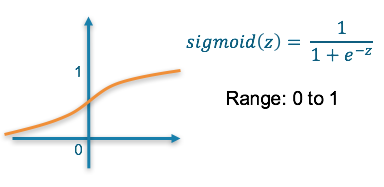
\includegraphics[width=0.33\linewidth]{png/sigmoid}
   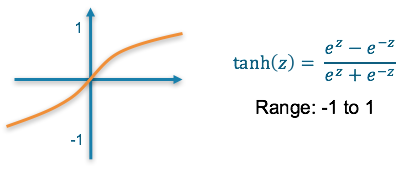
\includegraphics[width=0.33\linewidth]{png/tanh}
   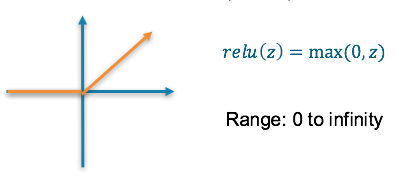
\includegraphics[width=0.33\linewidth]{png/relu}
   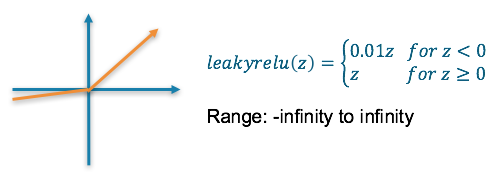
\includegraphics[width=0.33\linewidth]{png/leakyrelu}
  \caption{Activation functions. Source: \cite{stacey2018activation}.}
  \label{fig_activation} 
\end{figure}

	Activation functions also known as transfer functions are used to map input nodes to output nodes in certain fashion. Activation functions are extremely important for an ANN to learn and figure out features and characteristics of data which need a non-linear transformation to become outputs. There are the four most popular functions used in Deep Learning, their names are Sigmoid, Hyperbolic Tangent (Tanh), Rectified Linear Units (ReLU), Leaky ReLU and Exponential Linear Unit (ELU) (See in Fig. \ref{fig_activation}).

\begin{itemize}
\item \textbf{Sigmoid function}: takes a number as input and returns a value in $	[ \,0,1] \,$.
	$$f(x) = \frac{1}{1+e^x}$$
\item \textbf{Hyperbolic Tangent (Tanh) function}: is also like Sigmoid function but better, the range of the output from Tanh funtion is in $	[ \,-1,1] \,$.
 $$f(x) = \frac{2}{1+e^{-2x}} = 2\sigma(2x)-1$$
\item \textbf{Rectified Linear Unit (ReLU) function}: is a function having threshold at $0$ value. It helps accelerate the training process in ANN, so it is used in almost all the complicated deep learning models such as RNNs and CNNs.
$$f(x) = max(0, x)$$
\item \textbf{Leaky ReLU function}: is like ReLU function, but instead of setting thresholf value at $0$, Leaky ReLU extends the domain to $\alpha x$.
\[
    f(x)= 
\begin{cases}
    x,& \text{if } x > 1\\
    \alpha x, & \text{otherwise}
\end{cases}
\]
\end{itemize}
	
\subsection{Loss functions}
\label{ann_loss_func}
Neural Networks are trained by backpropagation algorithm, which updates the weights parameters of ANN according to a loss value. The loss value is calculated by a loss function, so loss functions are totally vital when an ANN model is built for learning information from data. These functions will essentially measure how poorly a model is performing by comparing what the model is predicting with the actual value it is supposed to output. Therefore, choosing a loss function that is appropriate for penalizing model effectively is one of the most important tasks while working with data. There are a number of loss functions for deep learning models, and each of them have its own pros and cons. The common loss functions that are widely used in time-series forecasting will be presented as below:
\begin{itemize}
\item  \textbf{Mean Absolute Error (MAE)}: 
$$MAE = \frac{\sum|e_t|}{N}$$
\item  \textbf{Sum Square Error (SSE)}: $$SSE = \sum(e_t^2)$$
\item  \textbf{Mean Square Error (MSE)}: $$MSE = \frac{\sum(e_t^2)}{N}$$
\item  \textbf{Root Mean Square Error (RMSE)}: $$RMSE = \sqrt{MSE}$$
\item  \textbf{Mean Absolute Percentage Error (MAPE)}: $$MAPE = \frac{1}{N}\sum|\frac{e_t}{y_t}|$$
Where $N$ is the number of data points, $y_t$ is the actual output value, $d_t$ is the output value predicted by models, $e_t = d_t - y_t$ is the error value of the data point $t$.
\end{itemize}
	 
\subsection{Backpropagation - the ANN Training Algorithm}
\label{ann_backprop_alg}

\begin{algorithm}[!t]
	\caption{Backpropagation algorithm applied for FFNN with 1 hidden layer}
	\label{algorithm_backprop}
	\SetAlgoLined
	Initialize randomly weights' value $w_p$\\ 
	\Repeat{Until convergence or the number of iterations is enough}{
	\textbf{Calculate output value(s) according to weights and input}  \\
	
		\For{$j= 1$ to $h$}
		{
			$H_{j} = \phi(\sum_i^n {x_i*w_{ij}^{[1]} + b_{ij}^{[1]}})$ \\ 
			
		}
		$\widehat {{y_j}} = \phi(\sum_i^h{H_i * w_j^{[2]} + b_j^{[2]}})$\\
		
		\textbf{Calculate Loss value by loss function} \\ 
		
		$L(w) = loss(\widehat {{y_j}},{y_j})  $ \\
		
		 \textbf{Backpropagating Loss to weights}\\
		
		$ \bigtriangleup(w_{ij}^2) = \frac{\partial (L(w))}{\partial (w_{ij}^2)}$ \\
		$ \bigtriangleup(w_{ij}^1) = \frac{\partial (L(w))}{\partial (w_{ij}^1)}$ \\
		
		\textbf{Update weights' value} \\ 
		
		$w_{ij}^2 = w_{ij}^2 - \eta * \bigtriangleup(w_{ij}^2)$ \\
		$w_{ij}^1 = w_{ij}^1 - \eta * \bigtriangleup(w_{ij}^1)$
	}
		
\end{algorithm}

Back-propagation algorithm is undoubtedly the most fundamental building block in an ANN. It It was first introduced in 1960s and almost 30 years later (1989) popularized by Rumelhart, Hinton and Williams in~\cite{rumelhart1988learning}. The algorithm is used to effectively train a neural network through a method called chain rule. In simple terms, after each forward pass through a network (propagation phase), back-propagation performs a backward pass while adjusting the model's parameters (weights and biases) (weights updating phase).

\subsubsection{Forward propagation phase}
\begin{enumerate}
\item The input values will be fed into ANN through input layer, going forward to hidden layers, and finally to output layer, creating predicted output values. While propagation process, each layer uses its own activation function (sec. \ref{ann_act_func})
\item Error values are calculated by the loss function and propagated back to previous layers.
\end{enumerate}
\subsubsection{Weights updating phase}

\begin{enumerate}
\item Calculating gradients of loss function in weights and biases following the chain rule.
\item Updating weights and biases is done according to gradients' values 
\end{enumerate}

These two phases are repeated in each iteration during training. The algorithm will be stopped when the error from loss function reach a acceptable value or when the training iteration is large enough. The algorithm's pseudo code is presented in short in Algorithm \ref{algorithm_backprop}.

\subsection{Well-known machine learning models for time-series prediction problem}
\label{wl_known_models}

	Recent developments in cloud computing including resource management have resulted in a significant interest in resource usage prediction . Various traditional methods such as Autoagressive model (AM), Autoregressive Moving Average (ARMA), Autoregressive Integrated Moving Average (ARIMA) and General Autoregressive Conditional Heteroscedastic (GARCH) have been proposed for solving this problem with different aspects, objectives and applications ~\cite{amiri2017survey}. In this section, we focus on several Artificial Neural Network (ANN) models that are used for learning the time-series characteristic of sequence data.
	Deep Feed-forward Neural Network, also called Feed-forward Neural Network (FFNN) are the quintessential deep learning models. The goal of all FFNN is to approximate some functions $f^*$.  In Regression problems, $y = f^*(x)$ maps an input $x$ to a value $y$. A feed-forward network defines a mapping $y = f(x,\theta)$ and learns the value of the parameters $\theta$ that result in the best function approximation. ~\cite{Goodfellow-et-al-2016}. These models are called feed-forward because information flows through the function being evaluated from $x$, through the intermediate computations used to define $f$, and finally to the output $y$. There are no feedback connections in which outputs of the model are fed back into itself. When feed-forward neural networks are extended to include feedback connections, they are called recurrent neural networks, which will be discussed in ~\ref{model_rnn}.
	
	In general, Multi-Layer Perceptrons (MLPs) models contain several disparate layers. The first layer is input layer taking information $x$ as input for the network. The last layer is called output layer, whose value is the result of $y$ with input $x$. The layers between the input and output layers are hidden layers. The structures of hidden layers are extremely diverse, varying from model to model. As presented in Fig. \ref{fig_model_mlp}, a hidden layer of a simple FFNN is a group of neurons with no connection to each other, while in Recurrent Neural Networks (RNN), and Convolution Neural Network (CNN) hidden layer is a recurrent layer, and convolution layer respectively. 
	
	The Deep Neural Networks that are applied for Time series prediction will have input neurons presenting the historical data. The models utilize information from data in the past for forecasting future data. Input data presented as $x_1, x_2, ..., x_t$ is considered as historical values up to time t, which is used to predict the value at the time $t+1$. In other words, Deep Neural Networks will learn from data and approximate a function transforming the historical data up to time $t$ to the data at the time $t+1$ as follows:
\begin{equation} \label{eq_ffnn_1}
x(t+1) = y = f(x_1, x_2, ..., x_t)
\end{equation}
	
	 In this section, we summarize several Deep Neural Network models, which are widely used for time series forecasting. They are simple Multi-Layer Perceptrons (MLPs), Cascade Forward Neural Network (CFNN) and Recurrent-based Neural Network including traditional Recurrent Neural Network (RNN), Long-Short Term Memory (LSTM) and Gated Recurrent Units (GRU). Each method will be presented below with brief ideas and mathematical formulas. 

\begin{figure}[!ht] 
   \centering
   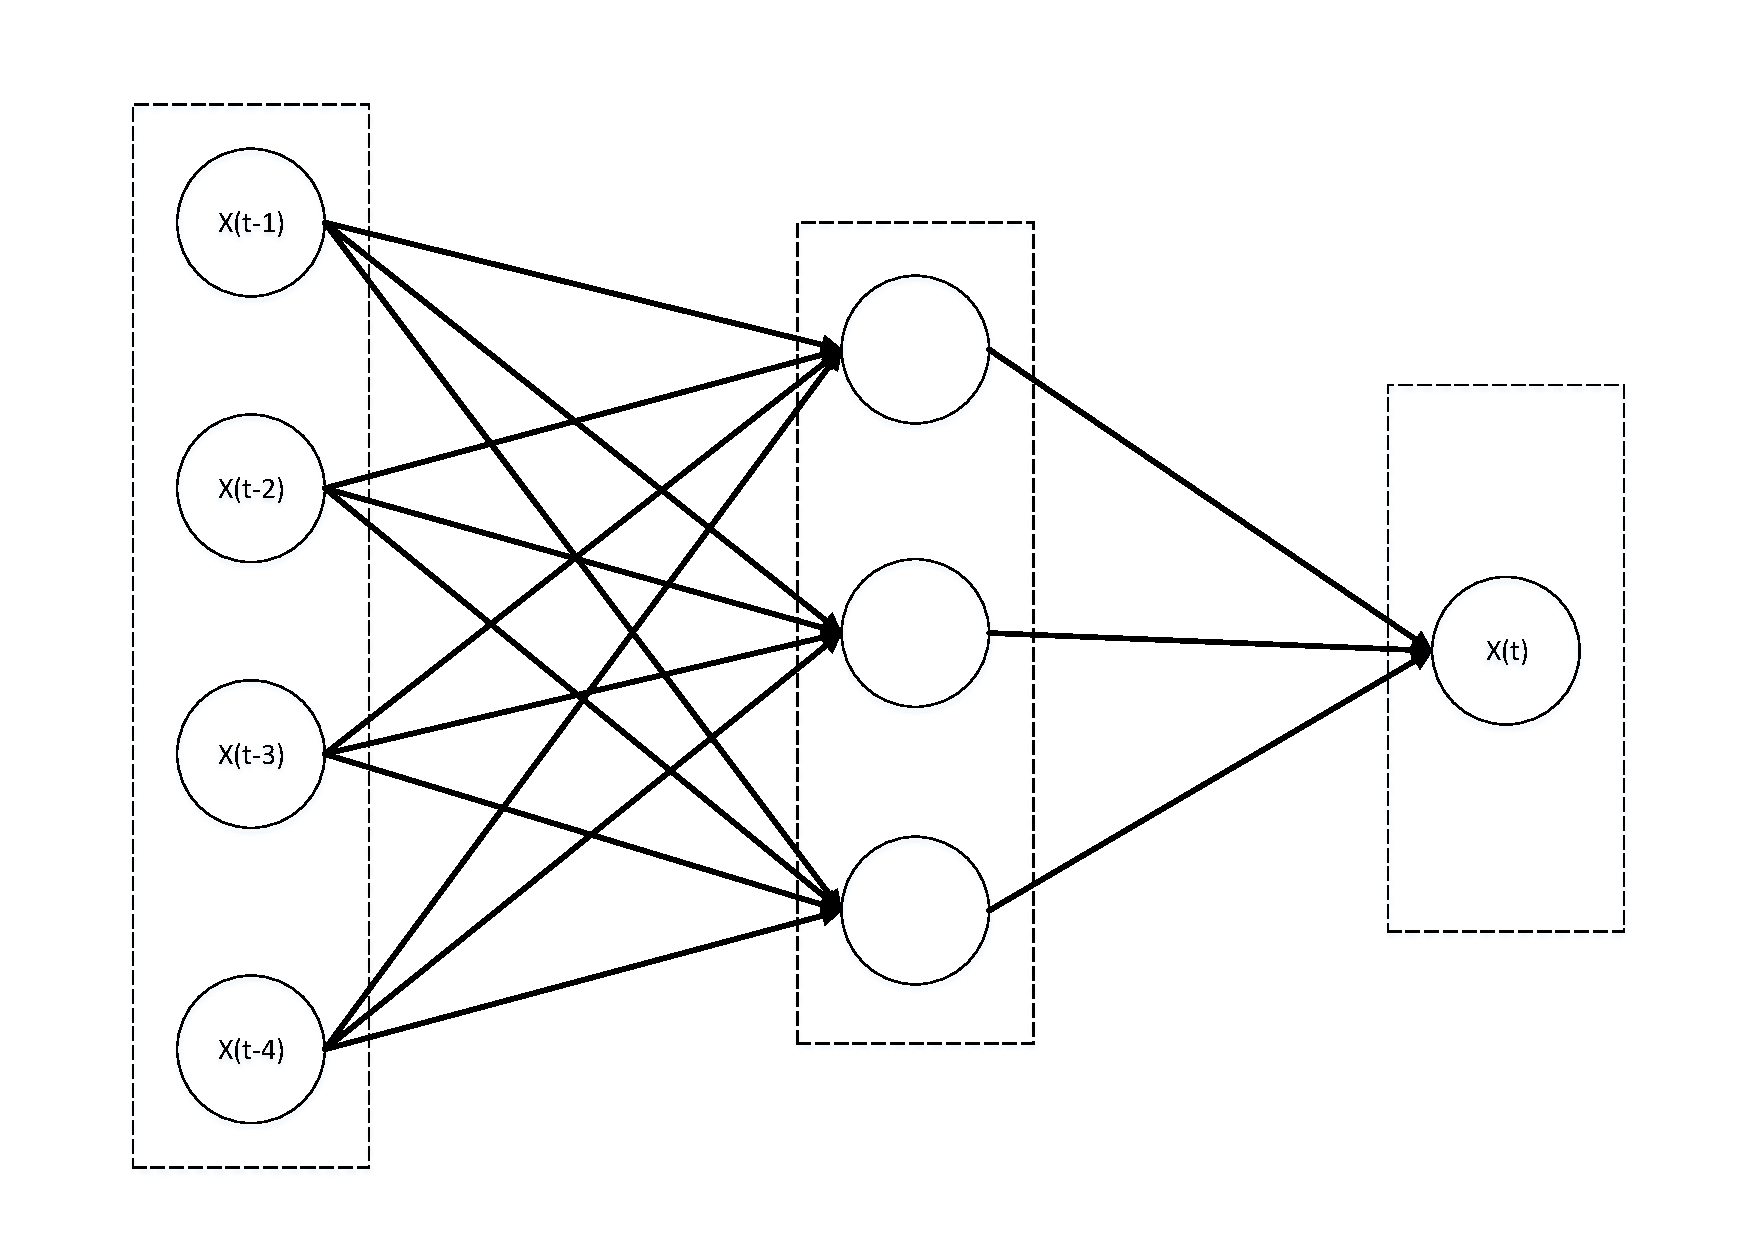
\includegraphics[width=0.75\linewidth]{pdf/model/model_ffnn}
  \caption{An example of MLPs model in time-series prediction.} 
  \label{fig_model_mlp} 
\end{figure}

\subsubsection{Multi-Layer Perceptrons (MLPs)}
\label{model_mlp}
	
	The additional layers added between input layer and output layer make network architecture contain hidden layers and called Multi-Layer Perceptrons (MLPs). The input data is fed through input layer to hidden layers in the weighted form. The information from input data $X$ is distributed to the neurons in hidden layers and then processed by an activation function. The activation function in hidden layers are non-linear function playing a role as a transfer function, helping MLPs learn non-linear characteristics of the data. The information after being processed by hidden layers then are sent to output layer in the weighted sum, and also go through an activation function as well, creating the output value $y$. MLPs model is used in predicting time series data ~\cite{azoff1994neural}, ~\cite{koskela1996time}.  Fig. \ref{fig_model_mlp} shows a MLPs with a 4-neuron input layer and one output layer. In general,  the mathematical equation of the MLPs architecture can be written as follows:
\begin{equation} \label{eq_mlp_1}
H = f_h(W_h^TX + b_h)
\end{equation}
\begin{equation} \label{eq_mlp_2}
y = O = f_o(W_o^TH + b_o
\end{equation}

Where $X$ is the input data, $H$ and $O$ are the information after being fed through the hidden and output layers. $W_h$, $b_h$ and $W_o$, $b_o$ are weights and biases, while $f_h$ and $f_o$ are activation functions of hidden layer and output layer, respectively.


\subsubsection{Cascade Forward Neural Network (CFNN)}
\label{model_cfnn}

The main difference between CFNN and MLPs is that in CFNN, perceptron connection is added directly between neurons in input layer and output layer, while in MLPs, that connection is indirect through the hidden layer. The output layer of CFNN perceives both transformed information that is output of hidden layer, and the raw information from input data. This Deep Neural Network model was first used for forecasting monthly palm oil price in the Europe market in ~\cite{warsito2018cascade}. The architecture of CFNN with 4-neuron input layer is illustrated in Fig. \ref{fig_model_cfnn}, and the mathematical formulas for CFNN model are presented as follows:
\begin{equation}\label{eq_cfnn_1}
H = f_h(W_h^TX + b_h)
\end{equation}
\begin{equation}\label{eq_cfnn_2}
C = f_c(W_c^TX) + b_c
\end{equation}
\begin{equation}\label{eq_cfnn_3}
y = O = f_o(W_o^TH + b_o) + C
\end{equation} 
where $f_c$ is the activation function from the input layer to output layer, $C$ is the output value of $f_c$, and $W_c, b_c$ are weights and biases of the connection, respectively.

\begin{figure}[!ht] 
   \centering
   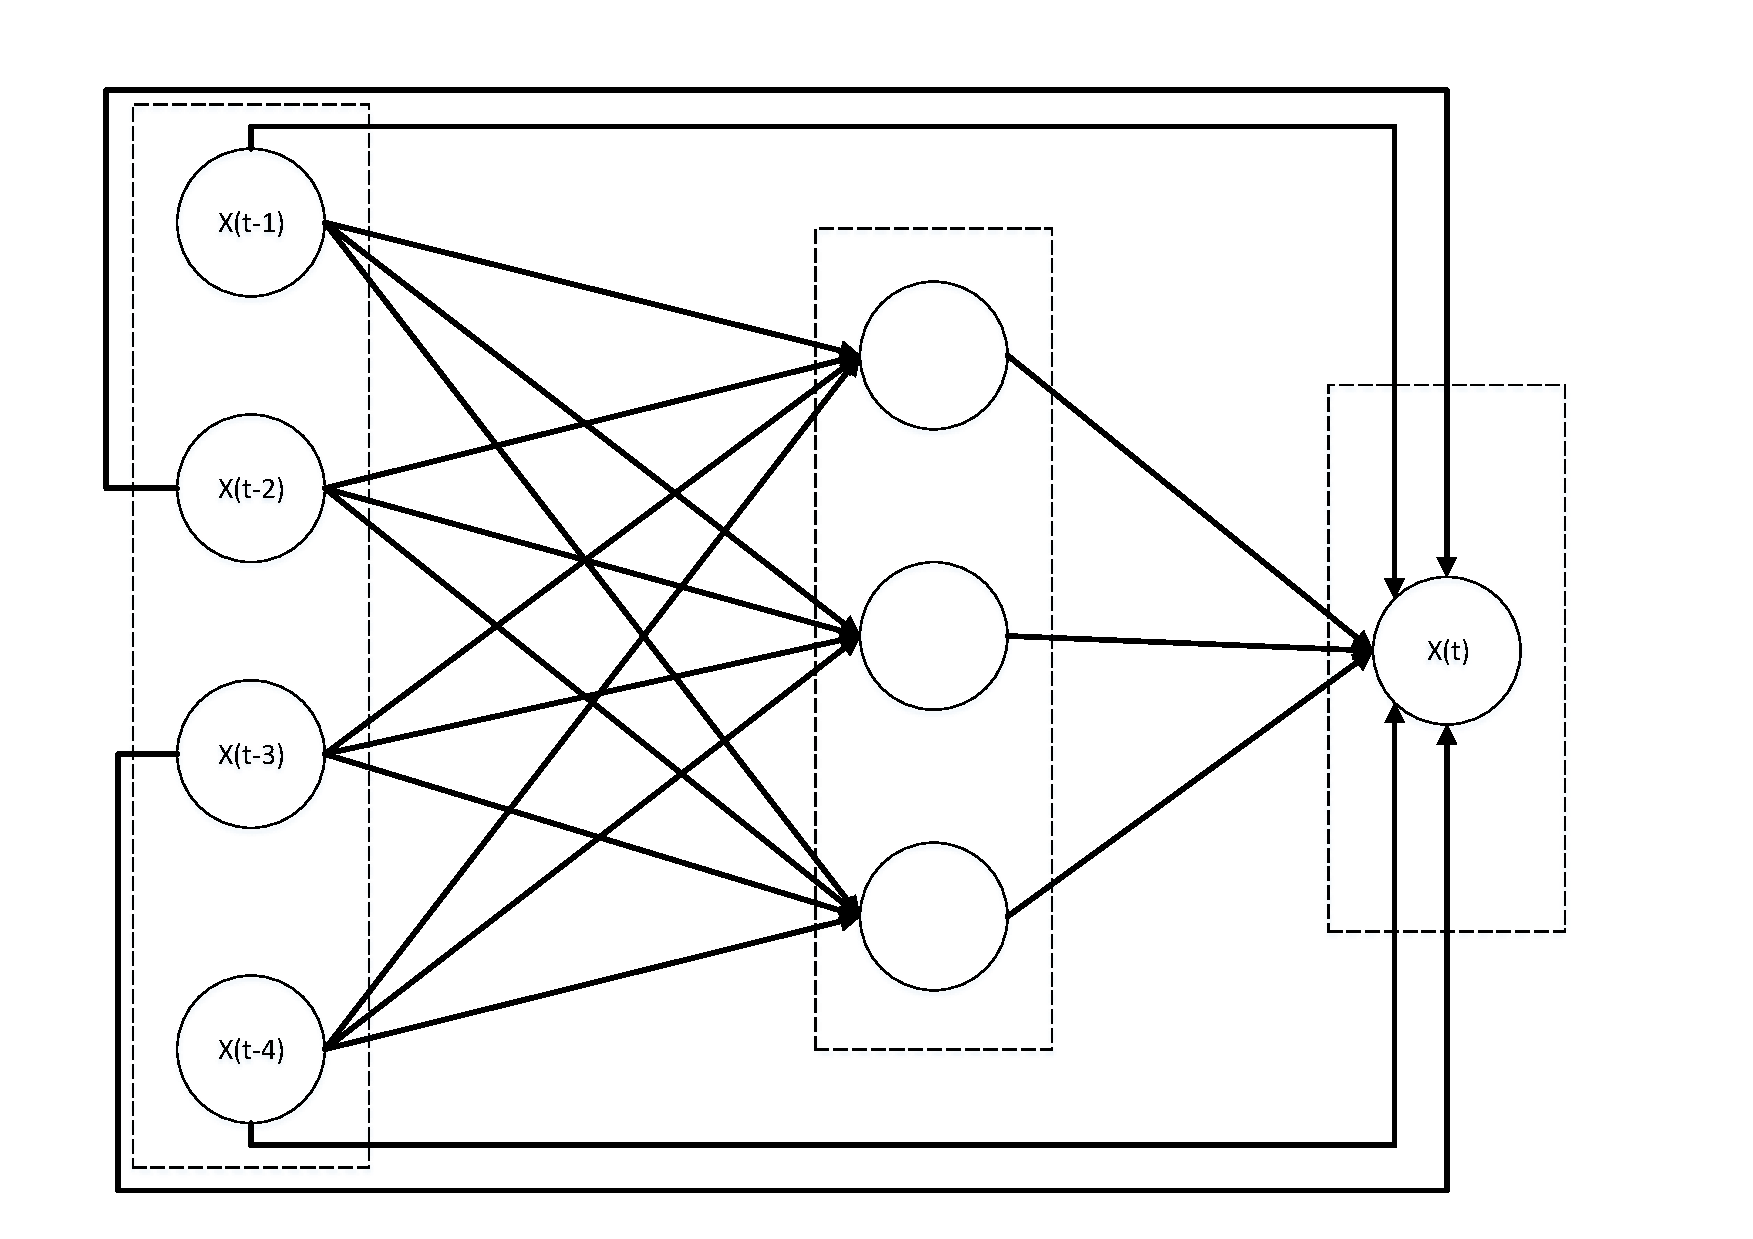
\includegraphics[width=0.75\linewidth]{pdf/model/model_cfnn}
  \caption{An example of CFNN model in time-series prediction.} 
  \label{fig_model_cfnn} 
\end{figure}


\subsubsection{Recurrent Neural Network (RNN)}
\label{model_rnn}
	Recurrent neural networks (RNNs) are dynamical systems that are specifically designed for temporal problems, as they have both feed-back and feed-forward connections (Fig. \ref{model_rnn}). RNN remembers the past and  its decisions are influenced by what it has learned from the past. RNNs can take one or more input vectors and produce one or more output vectors and the output(s) are influenced not just by weights applied on inputs like a regular MLPs, but also by a state vector representing the context based on prior input(s)/output(s),  so the same input could produce a different output depending on previous inputs in the series. For that reason, RNN is one of the most popular models being used for modeling time series data~\cite{zhang2000predicting},~\cite{connor1994recurrent},~\cite{chandra2012cooperative}. There are two popular and efficient RNN models that work really well: Long Short-Term Memory (LSTM) and Gated Recurrent Unit (GRU) which are discussed below. 
\begin{figure}[!ht] 
   \centering
   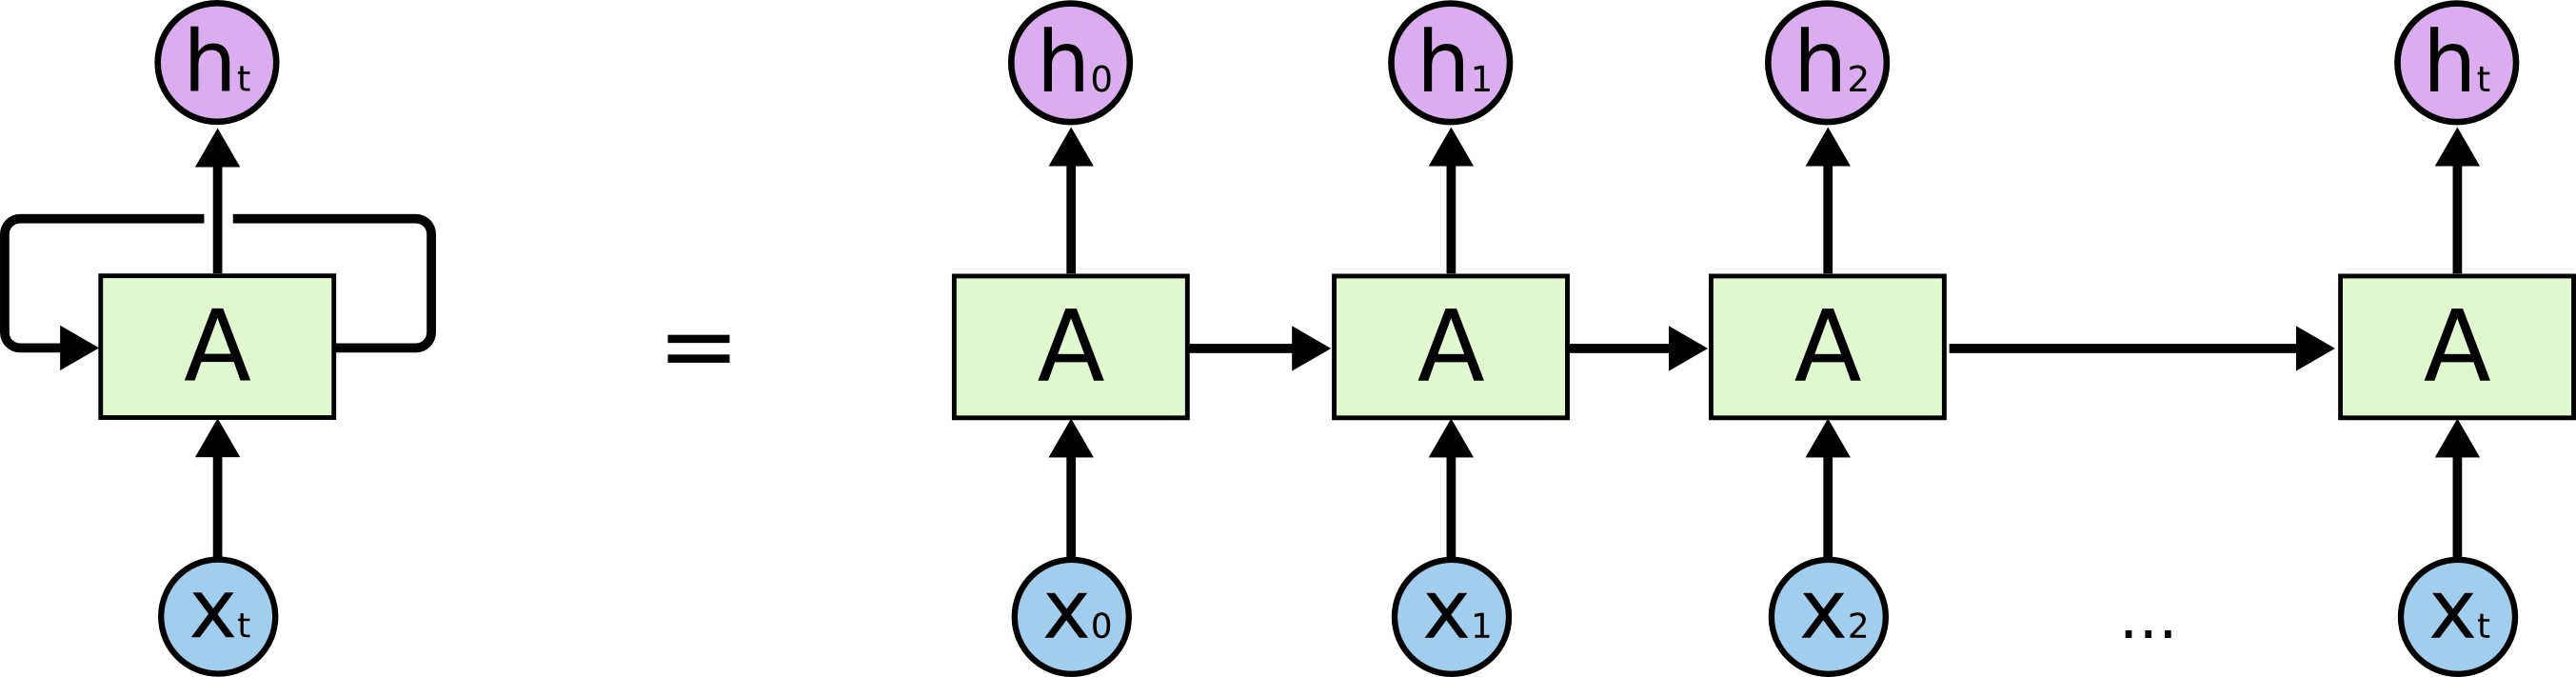
\includegraphics[width=1.0\linewidth]{png/rnn_unrolled}
  \caption{Traditional RNN architechture. Source: \cite{chris2015lstm}} 
  \label{model_lstm_gru} 
\end{figure}

\subsubsection{Long Short-Term Memory (LSTM)}
	Long short-term memory (LSTM)~\cite{hochreiter1997long} is a special kind of RNN created for learning long-term dependencies. LSTM units have 3 gates managing the contents of the memory. These gates are simple logistic functions of weighted sums, where the weights might be learnt by backpropagation. It means that, even though it seems a bit complicated, the LSTM perfectly fits into the neural network and its training process. With combining a forget gate in LSTM units, LSTM is capable to determine what it needs to remember and forget, so LSTM can work very well with dependent data , especially with time series data ~\cite{gers2002applying}, ~\cite{guo2016robust}, ~\cite{fu2016using}. The architecture of LSTM units is illustrated in Fig. \ref{model_lstm_gru}, and its mathematical model is briefly described as follows:
	 The input gate (\ref{eq_lstm_1}) and the forget gate (\ref{eq_lstm_2}) manage the cell state (\ref{eq_lstm_4}), which is the long-term memory. The output gate (\ref{eq_lstm_3}) produces the output vector or hidden state (\ref{eq_lstm_5}), which is the memory focused for use. This memory system enables the network to remember for a long time, which was badly missing from vanilla recurrent neural networks. 
\begin{equation}\label{eq_lstm_1}
i_t = sigmoid(W_ix_t + U_ih_{t-1}+b_i)
\end{equation}
\begin{equation}\label{eq_lstm_2}
f_t = sigmoid(W_fx_t + U_fh_{t-1}+b_f)
\end{equation}
\begin{equation}\label{eq_lstm_3}
o_t = sigmoid(W_ox_t + U_oh_{t-1}+b_o)
\end{equation}
\begin{equation}\label{eq_lstm_4}
c_t = f_t \odot c_{t-1} + i_t \odot tanh(W_cx_t + U_ch_{t-1} + b_c)
\end{equation}
\begin{equation}\label{eq_lstm_5}
h_t = o_t \odot tanh(c_t)
\end{equation}
\begin{figure}[!ht] 
   \centering
   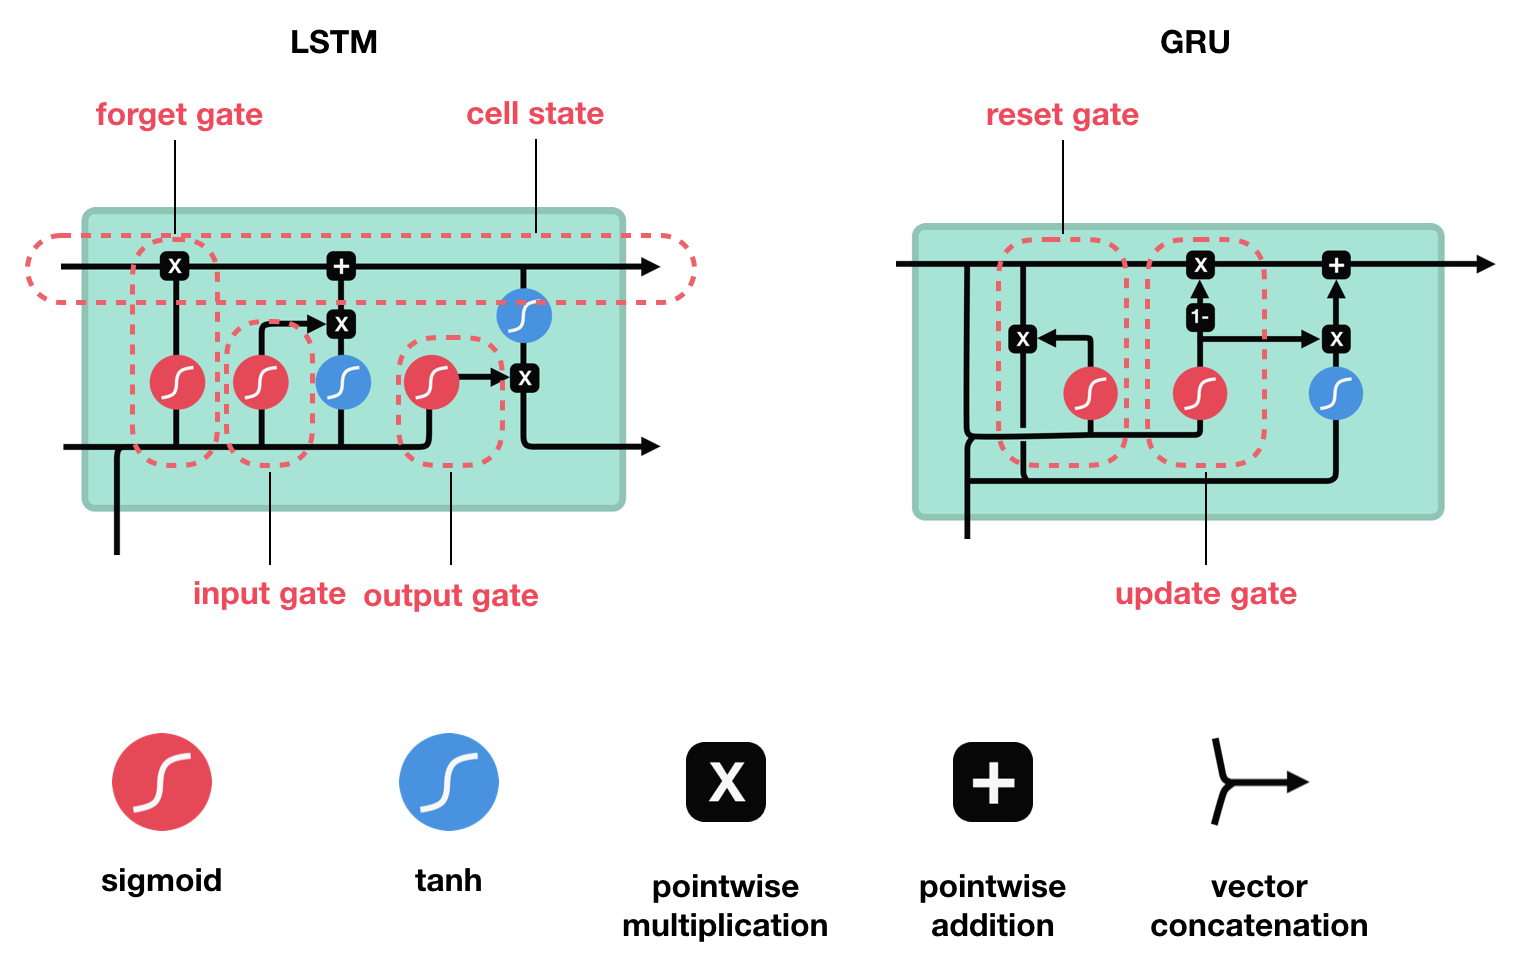
\includegraphics[width=1.0\linewidth]{png/lstm_gru}
  \caption{LSTM and GRU architechture. Source: \cite{michael2018lstm}} 
  \label{model_lstm_gru} 
\end{figure}

\subsubsection{Gated Recurrent Units (GRU)}

	Gated recurrent unit (GRU)~\cite{chung2014empirical} is essentially a simplified LSTM. Different form LSTM, GRU uses two gated called update gate and reset gate. Basically, these gates are two vectors managing what information should be passed to the output. In GRU, its gates can be trained to keep information from long ago, without washing it through time or remove information which is irrelevant to the prediction. It has the exact same role as LSTM in the network. The main difference is in the number of gates and weights - GRU is somewhat simpler. Like LSTM, GRU is also a widely chosen solution for time series forecasting such as in~\cite{langkvist2014review} and~\cite{bone2000recurrent} The srtucture of GRU units is presented in Fig. \ref{model_lstm_gru} following the mathematical model as below:
	
	The update gate~\ref{eq_gru_1} controls the information flow from the previous activation, and the addition of new information as well~\ref{eq_gru_3}, while the reset gate~\ref{eq_gru_2} is inserted into the candidate activation. Overall, it is pretty similar to LSTM. From these differences alone, it is hard to tell, which one is the better choice for a given problem. 
\begin{equation}\label{eq_gru_1}
z_t = sigmoid(W_zx_t + U_zh_{t−1} + b_z)
\end{equation}
\begin{equation}\label{eq_gru_2}
r_t = sigmoid(W_rx_t + U_rh_{t−1} + b_r)
\end{equation}
\begin{equation}\label{eq_gru_3}
h_t = z_t\odot h_{t-1} + (1 - z_t)\odot tanh(W_hx_t + U_h(r_th_{t-1}) + b_h)
\end{equation}

\section{Auto-scaling problem in Cloud Computing}
\label{sec:application}

\subsection{Cloud Computing}
\label{cloud}
	Cloud technology has evolved from the costly and complex information technology (IT)
solutions and enterprise applications in the 1980s, and is enabled by the recent expansion of the Internet in the 1990s. Moreover, the dramatic drop in the bandwidth costs and other technological advances have contributed to the emergence of cloud computing \cite{mell2011nist}. Unlike previous generations of application service providers (ASPs), cloud computing
provides tangible and measurable business benefits by allowing multi-user-real-time access without the up-front investment cost. In general, cloud computing is a computing paradigm, where a large pool of systems are connected in private or
public networks, to provide dynamically scalable infrastructure for application, data and file storage. With the advent of this technology, the cost of computation, application hosting, content storage and delivery is reduced significantly. Cloud computing is a practical approach to experience direct cost benefits and it has the potential to transform a data center from a capital-intensive set up to a variable priced environment.

\begin{figure}[!ht] 
   \centering
   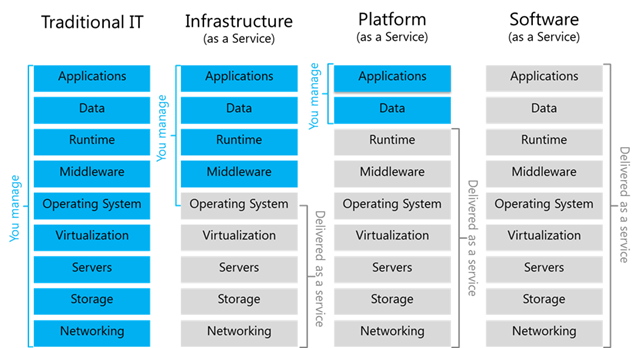
\includegraphics[width=1.0\linewidth]{/png/cloud_models}
  \caption{Comparision between Traditional IT and three models of Cloud computing. Source: \cite{david2018cloud})} 
  \label{fig_cloud_models} 
\end{figure}


	Cloud Providers offer services that can be categorized into three categories (See Fig. \ref{fig_cloud_models}):
\begin{enumerate}
\item \textbf{Software as a Service (SaaS):} In this model, a complete application is offered to customers as a service running on demand. A single instance of service runs on clouds, and multiple end users are served the same service. On the provider's side, the costs are lower since there is only one application that needs to be built and maintained, while in customers' side, there is no need for upfront investment in servers and software licenses. Today, there is a number of companies such as Google, Microsoft and Zoho playing a role as SaaS providers.
\item \textbf{Platform as a Service (Paas):} In this category, a layer of software, or a development environment is encapsulated and offered as a service, upon which high level of services can be built. Customers are free to build their own application running on the provider's infrastructure. PaaS
providers offer a predefined combination of OS and application servers, such as LAMP platform
(Linux, Apache, MySql and PHP), restricted J2EE, Ruby etc. Google‟s App Engine, Force.com,
etc are some of the popular PaaS examples.
\item \textbf{Infrastructure as a Service (Iaas):} Basic storage and computing capabilities are provided as standardized services over the network by Iaas. Servers, storage systems, networking equipment, data
centre space etc. are pooled and made available to handle workloads. The customer would
typically deploy his own software on the infrastructure. Some common examples are Amazon,
GoGrid, 3 Tera.
\end{enumerate}

\subsection{Auto-scaling demand in Cloud Computing.}
\label{auto_scale}
The popularity of on-demand cloud service has spurred the migration of increasing numbers of web applications to the cloud. One of the most attractive features for cloud web application providers is the ability to access computing
resource elastically (by scaling up or down) according to dynamic resource demands. In this scenario, providers only pay for resources that are consumed at a specific point in time, which if operated correctly, will result in less cost
and higher quality service than is achievable by hosting on standard hardware. Nevertheless, true elasticity and cost-effectiveness in the
pay-per-use cloud business model have not yet been achieved completely. The management of allocating cloud resource adaptively to on-demand requirements of an application called auto-scaling, can be very challenging. Resource
under-provisioning will unavoidably harm performance and cause Service Level Agreements (SLAs) violations, while resource over-provisioning will result in resource idle and cost waste. Therefore, the final objective of an auto-scaling mechanism is to automatically adjust acquired resources to minimize cost while satisfied the SLAs.

	To achieve this target, several methods have been proposed. They can be divided into three groups of methods: Periodicity, Threshold and Prediction. Periodicity methods allow providers and customers to predefine time intervals, during which resource demands can be dilated or shrunk according to their experiences. The biggest drawback of this method is that system manager is unable to allocate suitable amount of resources when customer's requests come immediately. Unlike Periodicity, Threshold methods use lower bound L and upper bound U to define the minimum and maximum amount of resources that can be required. Adjusting resources is decided according to rules that are built by providers and customers. These methods face a problem of choosing suitable thresholds for satisfying resorces demand from applications. The third kind of methods, Prediction, is the most protential one. These methods use the information recorded over a period of time as time-series data to analyze and predict resources that can be required in the future. Since information collected have characteristics of time-series data, time-series forecasting models are usually used to tackle the workload predicting problem in cloud environment such as ARMA \cite{chen2015efficient}, \cite{yang2013workload} and ARIMA  \cite{calheiros2014workload}. However, traditional methods do not show competitive performance in term of accuracy. Recently, deep learning predicting models have been proposed for solving the workload predicting demand. The works in \cite{shahin2017automatic}, \cite{zhu2017deep} and \cite{tran2018multivariate} have proved that deep learning models such as simple FFNN, RNN, LSTM or GRU can provide very competitive results compared with other traiditional methods.  
	
	Nevertheless, there are several issues still remaining in these models. The main problem is of the BP algorithm being used to train NNs model, which are tendency being trapped in local minima, slow convergence and significant dependence on the initial stage of their parameters. Also, RNN-based models like LSTM and GRU are too complicated that can lead to overfitting, and contain a huge number of parameters to be optimized. Therefore in this work, we focus on solving the workload prediction demand by a simpler and more effective appoach: propose a model using meta-heuristic algorithm for optimizing a much less complicated NNs model: CFNN.
\end{document}